% Figures in this chapter
\newcommand{\Muscimol}{1}
\newcommand{\MuscimolDiagram}{\Muscimol A}
\newcommand{\MuscimolExample}{\Muscimol B}
\newcommand{\MuscimolSummary}{\Muscimol C}
\newcommand{\MuscimolSites}{2}
\newcommand{\FluorescentMuscimol}{3}
\newcommand{\MuscimolMovement}{4}
\newcommand{\MuscimolNumTrials}{\MuscimolMovement A}
\newcommand{\MuscimolCoutTime}{\MuscimolMovement B}
\newcommand{\MuscimolSideInTime}{\MuscimolMovement C}

\chapter{Striatal circuits are involved in sound frequency discrimination.}

\section{Author contributions}
\noindent Originally published as part of: Lan Guo, William I Walker, Nicholas D Ponvert, Phoebe L Penix, and Santiago Jaramillo, 2018.  Stable representation of sounds in the posterior striatum during flexible auditory decisions. \textit{Nature Communications} 9 (1534).
%
Santaigo Jaramillo provided mentorship for all aspects of the study. Nicholas D Ponvert performed all experiments included in this dissertation. Lan Guo, Nicholas D Ponvert, and Santiago Jaramillo wrote the sections of the paper pertaining to the results of the behavioral experiments included in this dissertation. 

\section{Introduction}
% DONE: This section mostly from the paper. I'm leaving it.
In the mammalian brain, the dorsal striatum links neural signals from the cerebral cortex to circuits in the basal ganglia to mediate action selection. Electrophysiological and inactivation studies have identified two regions within the dorsal striatum which play distinct roles in decision making: the dorsomedial striatum (DMS) involved in flexible goal-oriented behavior, and the dorsolateral striatum (DLS) which mediates habitual actions \citep{Yin2006, Balleine2009, Devan2011}.
%
Recent anatomical characterization of the excitatory input from cortex and thalamus onto the striatum suggests that the organization of the dorsal striatum goes beyond the DMS and DLS divide \citep{Hunnicutt2016}.
%
This characterization in rodents showed that the posterior portion of the striatum receives a combination of sensory inputs that sets it apart from other regions.
%
Similarly, an evaluation of reward-related signals of the dopaminergic input along the anterior-posterior axis of the striatum provides further evidence that the posterior tail of the striatum forms a circuit distinct from the anterior dorsal striatum, which includes the classically studied DMS and DLS regions \citep{Menegas2015, Menegas2017}.
%
It is not clear, however, whether the function of this posterior region is qualitatively different from the previously characterized striatal subregions.
%
Here, we evaluate the role of neurons in the posterior tail of the striatum during sensory-driven decisions in mice.

The posterior tail of the dorsal striatum in rodents (referred to hereafter as posterior striatum) receives direct neuronal projections from the auditory thalamus (ATh) and the auditory cortex (AC), as well as midbrain dopaminergic signals \citep{Menegas2015, Hunnicutt2016}.
%
Because of these anatomical features, this region is sometimes referred to as the auditory striatum \citep{Znamenskiy2013}.
%
Given this convergence of sensory and reward-related signals, and prompted by the role of other dorsal striatal regions, we hypothesized that the posterior striatum drives rewarded actions according to acoustic cues.

In this chapter, we train animals to perform a simple sound-frequency discrimination task, and then perform reversible inactivation of the posterior striatum to determine whether the region is necessary for task performance.
%
We observe strong deficits in task performance during sessions in which striatum was inactivated, supporting the hypothesis that this region plays a key role in tasks that require sound-action association.

\section{Methods}

\subsection{Animal subjects}
5 adult male wild-type mice (C57/BL6J) were used in this study. Mice had ad libitum access to food, but water was restricted. Free water was provided on days with no experimental sessions. All procedures were carried out in accordance with National Institutes of Health standards and were approved by the University of Oregon Institutional Animal Care and Use Committee.

\subsection{Behavioral task}
Behavioral data was collected using the taskontrol platform (\url{www.github.com/sjara/taskontrol}) developed in our laboratory using the Python programming language (\url{www.python.org}). Mice initiated each trial by poking their noses into the center port of a three-port behavior chamber. After a silent delay of random duration (150-250 ms, uniformly distributed), a narrow-band sound (chord) was presented for 100 ms. Animals were required to stay in the center port until the end of the sound and then chose one of the two side ports for reward (2 ul of water) according to the frequency of the sound (low-frequency: left port; high-frequency: right port). If animals withdrew before the end of the stimulus, the trial was aborted and ignored in the analysis. Stimuli were chords composed of 12 simultaneous pure tones logarithmically spaced in the range f/1.2 to 1.2f for a given center frequency f. Within a behavioral session, we used 6 or 8 distinct center frequencies. The intensity of all sound components was set to the same value between 30-50 dB-SPL (changing from one trial to the next) during the initial training, but fixed during testing at 50 dB-SPL. Each behavioral session lasted 60 to 90 minutes.

\subsection{Muscimol inactivation}
Bilateral craniotomies were performed under stereotactic surgery over the posterior striatum (1.7 mm posterior to bregma, 3.55 mm lateral from midline) of mice trained in the two-alternative choice sound discrimination task. Headbars were implanted to allow for head-fixation. Each craniotomy was protected with a plastic ring and filled with silicon elastomer (Sylgard 170, Dow Corning). Animals were allowed to recover for at least 3 days before resuming behavioral training. Following recovery, implanted animals were trained on the sound discrimination task until they reached their pre-surgery performance level before beginning muscimol inactivation.

For intracranial injection, we used glass pipettes (5 ul Disposable Micropipettes, VWR) pulled and trimmed to an inner diameter of 15-20 micrometers at the tip. Animals were head-fixed and allowed to run on a wheel during the injection. Craniotomies were exposed by removing the silicon elastomer covering, and a glass pipette filled with reagent (either muscimol or saline) was lowered into the brain to a depth of 3.1mm from brain surface using a micromanipulator. A volume of 45 nl of muscimol (0.25 mg ml$^{-1}$, final dose of 11.25 ng per hemisphere) was injected under air pressure in each hemisphere at a rate of 90 nl min$^{-1}$.
%
Given the relationship between concentration and diffusion distance (from Fick's law) and previous reports of muscimol effects on neuronal activity \citep{Edeline2002}, we expect that by the first 10 minutes of the behavioral session, the effects of muscimol (50\% reduction in firing or more) will be confined to a volume smaller than 1 mm in diameter centered at the injection site. This volume matches well the extent of the posterior tail of the striatum (approx. 1 mm A-P, 0.6 mm M-L, 1.5 mm D-V) that receives auditory inputs \citep{Hunnicutt2016}.
%
The pipette was left in place for 60 seconds following the injection, then raised 0.5mm and left in place for another 60 seconds before being removed. Injection in the second hemisphere was always completed within 10 minutes of the first injection. The craniotomies were then protected with a new silicon elastomer cap, and the mouse was placed back into its home cage for 30 minutes before starting the behavior session. After collection of 4 saline sessions and 4 muscimol sessions, 45 nl of fluorescent dye (DiI, Thermo Fisher Scientific) was injected at the same injection coordinates. Animals were then perfused transcardially with 5\% paraformaldehyde, and brains were extracted and postfixed for 12-24 hours. Brains were then sliced (100 um) and imaged to verify the location of fluorescent dye injection.

Fluorescent muscimol (Muscimol, BODIPY TMR-X Conjugate, Thermo Fisher Scientific) was dissolved in phosphate-buffered saline to a final concentration of 0.5 mg ml$^{-1}$. We followed the same protocol for intracranial injection as for muscimol. The injection volume was 360 nl per hemisphere (final dose of 180 ng per hemisphere) to account for the larger molecular weight and reduced spread of fluorescent muscimol. As with muscimol injections, animals rested for 30 minutes before starting the behavior session. Animals were euthanized and transcardially perfused with 5\% paraformaldehyde within 1 hour of finishing behavioral testing. Brains were extracted and postfixed overnight, and sliced (100 um) to quantify spread of fluorescent muscimol.

\subsection{Analysis of behavioral data}

Psychometric curve fitting was performed via constrained maximum likelihood to estimate the parameters of a logistic sigmoid function (\url{http://psignifit.sourceforge.net}). Statistical comparisons were performed using non-parametric statistical tests with no assumption of normality. 

\section{Results}

%%%%% Section - Change in overall performance %%%%%%%%
To test whether the activity of posterior striatal neurons was required when performing the sound-discrimination task, we quantified task performance during bilateral reversible inactivation of  these neurons (\fig{\Muscimol}, \fig{\MuscimolSites}).
%
Injection of muscimol (a GABA-A receptor agonist) in the posterior striatum resulted in a consistent decrease in task performance compared to injection of saline as control (\fig{\MuscimolExample}).
%
The effect was observed in all mice tested (\fig{\MuscimolSummary}, $p<0.05$ for each mouse, Wilcoxon rank-sum test), and consisted of a flattening of the psychometric curve.
%
Repeated injections did not alter task performance across the saline sessions tested ($r=-0.24$, $p=0.75$, linear regression of accuracy on sessions).
%
These results were replicated using fluorescent muscimol to confirm that inactivation restricted to the posterior striatum affected task performance (\fig{\FluorescentMuscimol}).

%%%%% Section - Movement effects %%%%%%%%

%
As a result of muscimol inactivation, mice displayed slower withdrawals from the center port on average ($p<0.05$ for four out of five mice, Wilcoxon rank-sum test, \fig{\MuscimolCoutTime}).
%
A change in movement speed from the center port to the reward ports was observed in only one out of five mice ($p<0.05$, Wilcoxon rank-sum test, \fig{\MuscimolSideInTime}).
%
Even though animals displayed motor impairments during muscimol inactivation, they still performed hundreds of trials during each session (480$\pm$146 muscimol \emph{vs.} 733$\pm$86 saline, \fig{\MuscimolNumTrials}, $p<0.05$ for three out of five mice, Wilcoxon rank-sum test).
%
During inactivation sessions, some animals used a strategy in which they chose a reward port at random, while other animals displayed a strong bias to one side.
%
Both of these strategies resulted in an average performance close to chance level for the binary choice.

% TODO: I should use a figure that has a better description of the task here.
\begin{figure}[!p]
  \begin{center}
    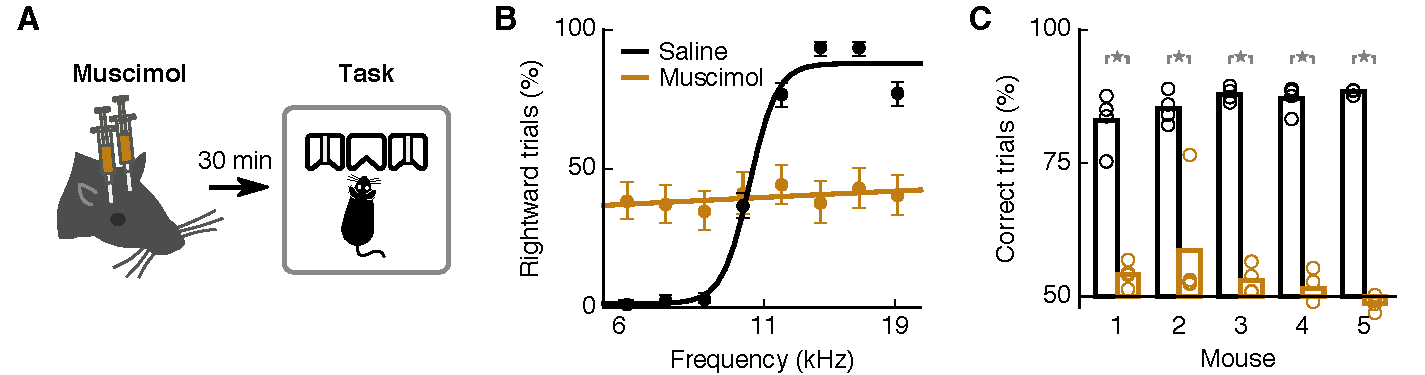
\includegraphics[width=5in]{figures/chapter2/Fig3_muscimol_inactivation}% 
  \end{center}
  \caption{Inactivation of posterior striatum impairs task performance.}{\textbf{(A)} Animals received bilateral injections of muscimol in the posterior
  striatum 30 minutes prior to starting the sound-frequency discrimination task. \textbf{(B)} During muscimol injection sessions (brown), animals performed significantly worse in the discrimination task than on days with control injections of saline (black). \textbf{(C)} Muscimol injection (brown) reduced performance to near chance level compared with saline injection (black) in all animals tested.}
\end{figure}


\begin{figure}[!p]
  \begin{center}
    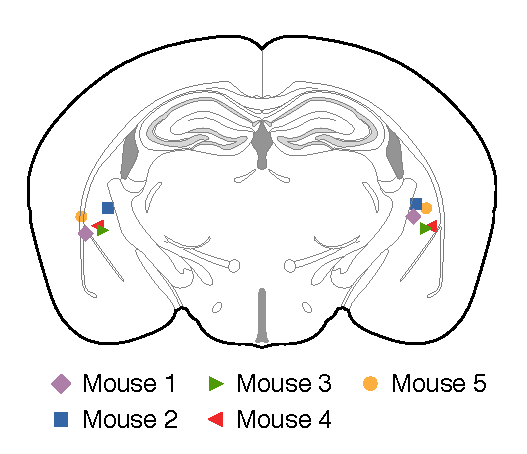
\includegraphics[width=3in]{figures/chapter2/SFig3_muscimol_injection_sites}% 
  \end{center}
  \caption{Location of muscimol injection sites.}{Injection sites were well-clustered and primarily contained to the posterior striatum.}
\end{figure}


\begin{figure}[!p]
  \begin{center}
    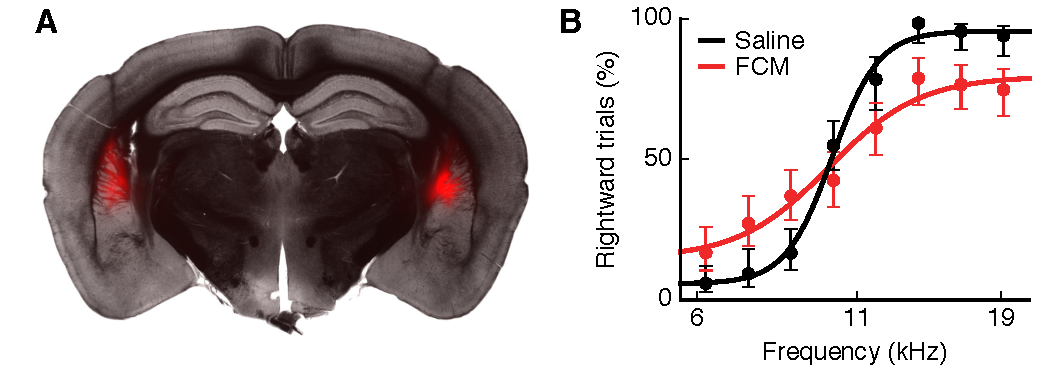
\includegraphics[width=5in]{figures/chapter2/SFig4_muscimol_inactivation_fluorescent}% 
  \end{center}
  \caption{Fluorescent muscimol well-restricted to posterior striatum causes reduction in task performance.}{\textbf{(A)} Muscimol conjugated with the fluorescent marker BODIPY was injected in the posterior striatum. In a histological section taken immediately after the behavior session, the extent of the muscimol injection is visible. \textbf{(B)} Injection of fluorescent muscimol affects discrimination performance in the frequency discriminaton task.}
\end{figure}



\begin{figure}[!p]
  \begin{center}
    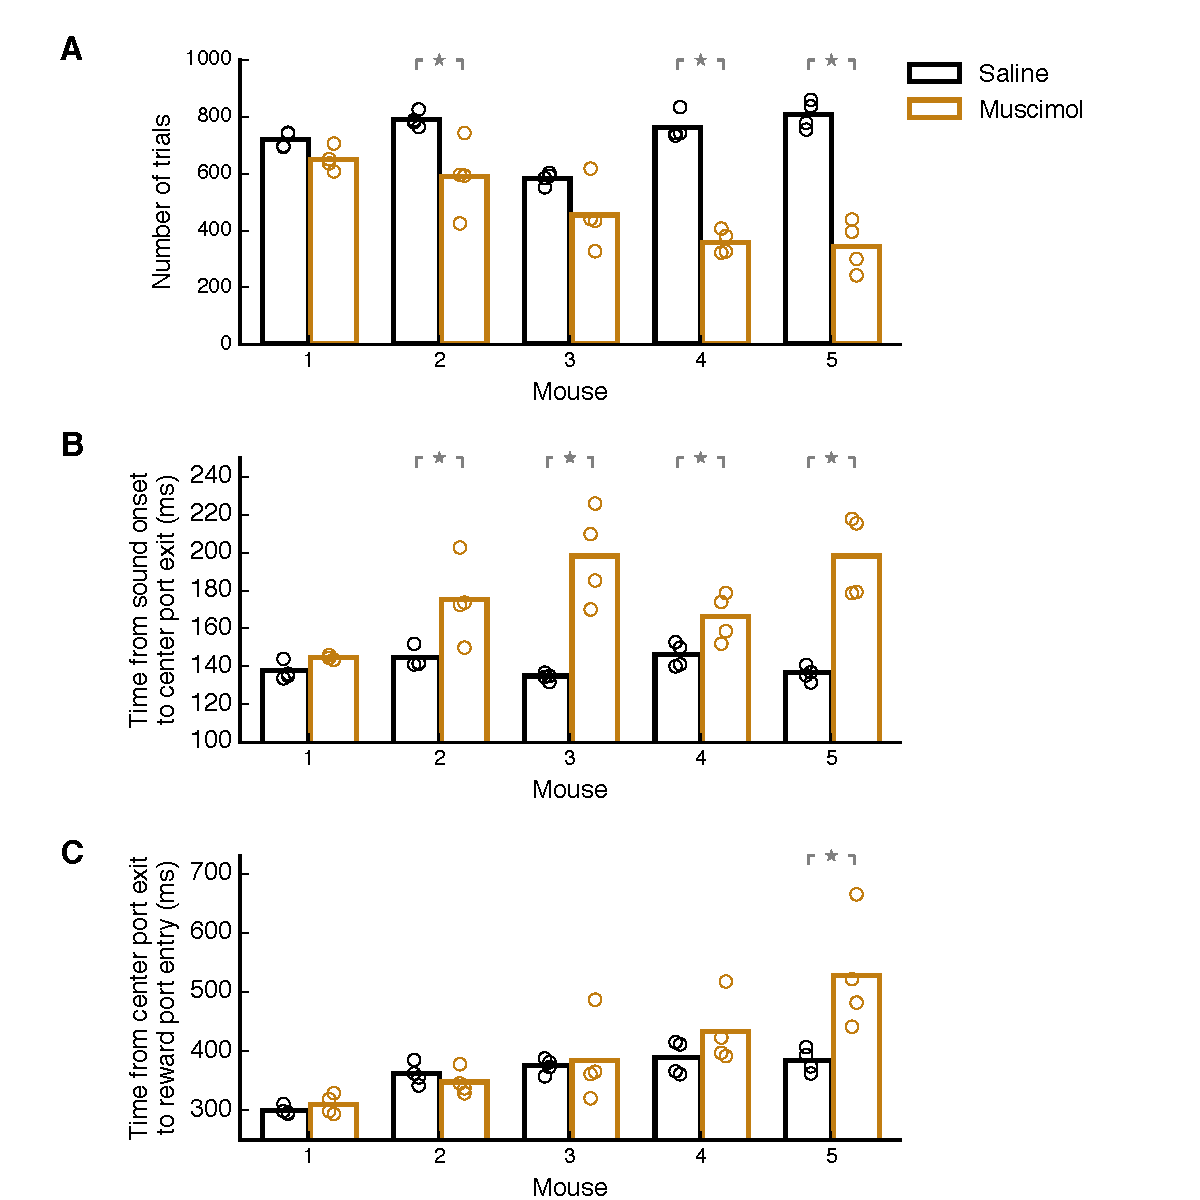
\includegraphics[width=5in]{figures/chapter2/SFig5_muscimol_inactivation_numtrials}% 
  \end{center}
  \caption{Inactivation of posterior striatum causes minimal motor impairment.}{\textbf{(A)} Three out of five animals tested performed significantly fewer trials in behavior sessions following muscimol injection (brown) compared to saline injection (black). \textbf{(B)} The delay between when the animal heard the sound and when it withdrew from the center port was significantly longer after muscimol injection for 4 out of 5 animals. \textbf{(C)} Only 1 out of 5 animals took longer to reach the side port after withdrawing from the center port.}
\end{figure}

\section{Discussion}

% This stuff is consistent with Zador lab stuff.
Recent studies of the corticostriatal pathway have proposed a model in which learning increases the efficacy of the synapses between neurons in auditory cortex that represent an auditory stimulus and neurons in the striatum that promote the action the animal should take after hearing that sound in order to get a reward \citep{Znamenskiy2013, Xiong2015}.
%
% DONE: A little more detail about the rest of the results in the paper here, but not much.
While the inactivation experiments described in this chapter are consistent with this model,  it does not fully account for other results described in \citet{Guo2018}.
%
For instance, in experiments where the categorization boundary was changed during the course of a single behavior session, requiring animals to switch the action associated with a particular stimulus, the sound responses of the large majority of posterior striatal neurons remains stable. 
%
If the sound-action association was encoded in the strength of the synapses between auditory areas and the posterior striatum, then the sound-evoked responses of posterior striatal neurons would be expected to change when the animal adapts to a new stimulus-action association.
%
Instead, the results of this study were more consistent with posterior striatal neurons providing information about the identity of the auditory stimulus, without considerable modulation by the subsequent choice. 

Our inactivation experiments demonstrate that silencing auditory striatal neurons has a drastic effect on a task that requires sound-driven decisions.
%
One interpretation of these results states that these neurons belong to a unique pathway required for successful performance of the frequency discrimination task we study.
%
Alternatively, these neurons could form one of several parallel pathways linking sensation to action, and reversible inactivation yields strong effects on behavior by altering the dynamics of downstream circuits.
%
Our experiments cannot distinguish between these possibilities, yet, provide strong support for a role of these striatal neurons in sensory-driven decisions.






In contrast with stimulation of anterior striatal regions, optogenetic stimulation of posterior striatal neurons did not elicit movements. 
%
On the other hand, we did find that chemical inactivation of the posterior striatum resulted in some motor effects.
%
However, motor impairment alone does not account for the performance deficits
observed during muscimol injection.
%
% TODO: Verify this number and the one below. 
In fact, only one animal tested took significantly longer to reach the side
reward port after withdrawing from the center port.
%
% TODO: So what?
Three animals tested displayed a longer latency to withdraw from the center port
after hearing the sound during muscimol sessions. 
%
% TODO: Come back to this sentence
Additionally, the reduced trial number observed during muscimol sessions in 4 out of 5 animals tested could also be the result of animals becoming frustrated and disengaging from the task due to a reduction in the number of rewarded trials.

% Posterior striatum activation in/out of task

% Posterior striatum neural responses

% Posterior striatum not choosing actions necessarily, but may convey sound info
Overall, \citet{Guo2018} found that posterior striatal neurons largely convey a stable representation of sounds to downstream areas.

% Need to investigate the relationship between the two parallel input streams.
Unresolved is the question of how the sound responses of the neurons in the posterior striatum are formed from the parallel auditory corticostriatal and thalamostriatal inputs.
%
% TODO: Need to talk about convergence?

